\subsection{Vehicle Volume Counting}
\label{subsection:count_measure}

This component of the algorithm takes as input the tracked object data from the object tracking component and returns updated traffic data for vehicle volumes. 

\subsubsection{Counting}

Depending on the direction of travel relative to the image, that is, up or down vs side to side, a line is specified on the image which when passed by a tracked object triggers a vehicle to be counted. The direction of travel of the object is determined by averaging the vehicle's position history. Figure \ref{fig:count_lines} shows an example of a count line. Algorithm \ref{algorithm:count} details the process of determining if a vehicle has crossed a count line.

\begin{algorithm}
	\SetAlgoLined
	\KwInput{List of tracked objects, tracked} 
	\KwOutput{Updated vehicle volume statistics}
	
	
	\caption{Centroid re-assignment algorithm. \cite{adrian_rosebrock_vehicle_tracking}}
	\label{algorithm:count}
  \end{algorithm}

\begin{figure}[H]
	\centering
	\begin{subfigure}[b]{0.42\textwidth}
            \centering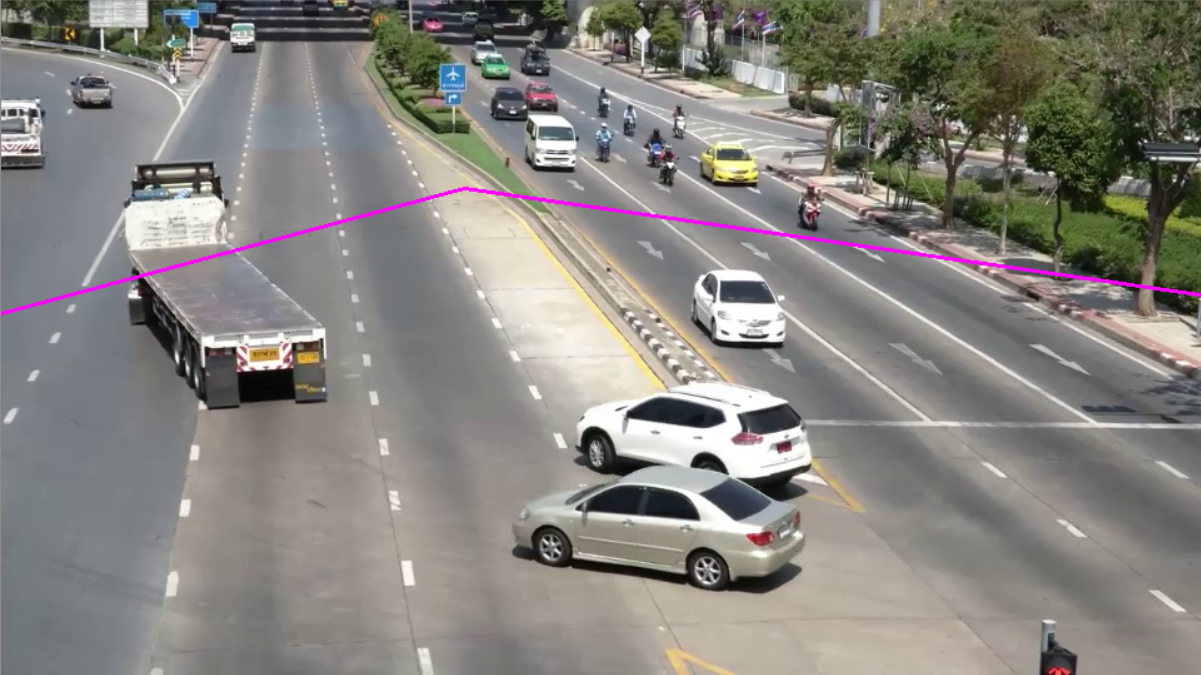
\includegraphics[width = \textwidth]{design/detection/counting/updowntraffic.png}|
            \captionsetup{format = hang}  
      		\caption{Count lines for traffic travelling up and down.}
    	\end{subfigure}
    	\begin{subfigure}[b]{0.42\textwidth}
      		\centering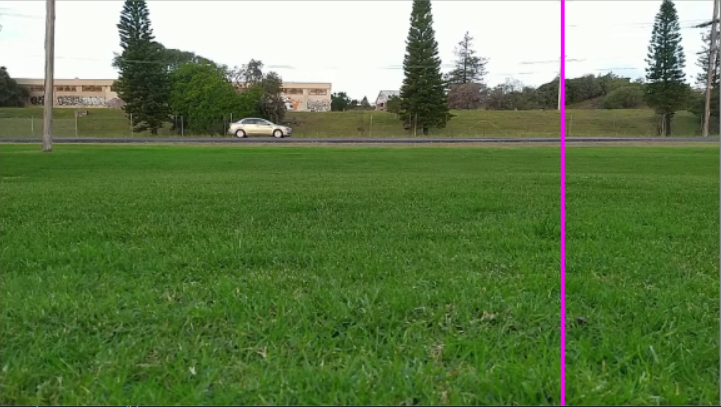
\includegraphics[width = \textwidth]{design/detection/counting/leftrighttraffic.png}
            \captionsetup{format = hang}    
            \caption{Count line for traffic travelling left and right.}
        \end{subfigure}
        \captionsetup{format = hang}
    	\caption{Count line visualization for both traffic direction orientations.}
    	\label{fig:count_lines}
\end{figure}

\subsubsection{Speed Estimation}

Time stamps associated with a vehicle's location history allow the speed of that vehicle to be estimated. Similar to when counting, two lines are placed on the image and when a vehicle travel between them it's speed over that region is measure. This is achieved by converting the distance travelled in pixels into meters. Figure \ref{fig:speed} shows an example highlighted region in which a vehicle's speed is measured.  For a camera perspective looking in the direction of travel as in Figure \ref{fig:original_frame} and not perpendicular to it, the accuracy will be reduced. This is because object scale changes with distance from a node. In a situation where vehicles are travelling perpendicular to the camera's perspective their size remains constant and hence perceived pixels per time unit doesn't change as they move. This type of speed measuring is referred to as \emph{Visual Average Speed Computer and Recorder} (VASCAR) as it relies on visual inputs to determine a vehicles speed, it is less accurate than other methods like radar but is sufficient for the purpose of measuring approximate traffic speed to gauge traffic flow in conjunction with vehicle volumes.

\begin{figure}[H]
	\centering
	\centering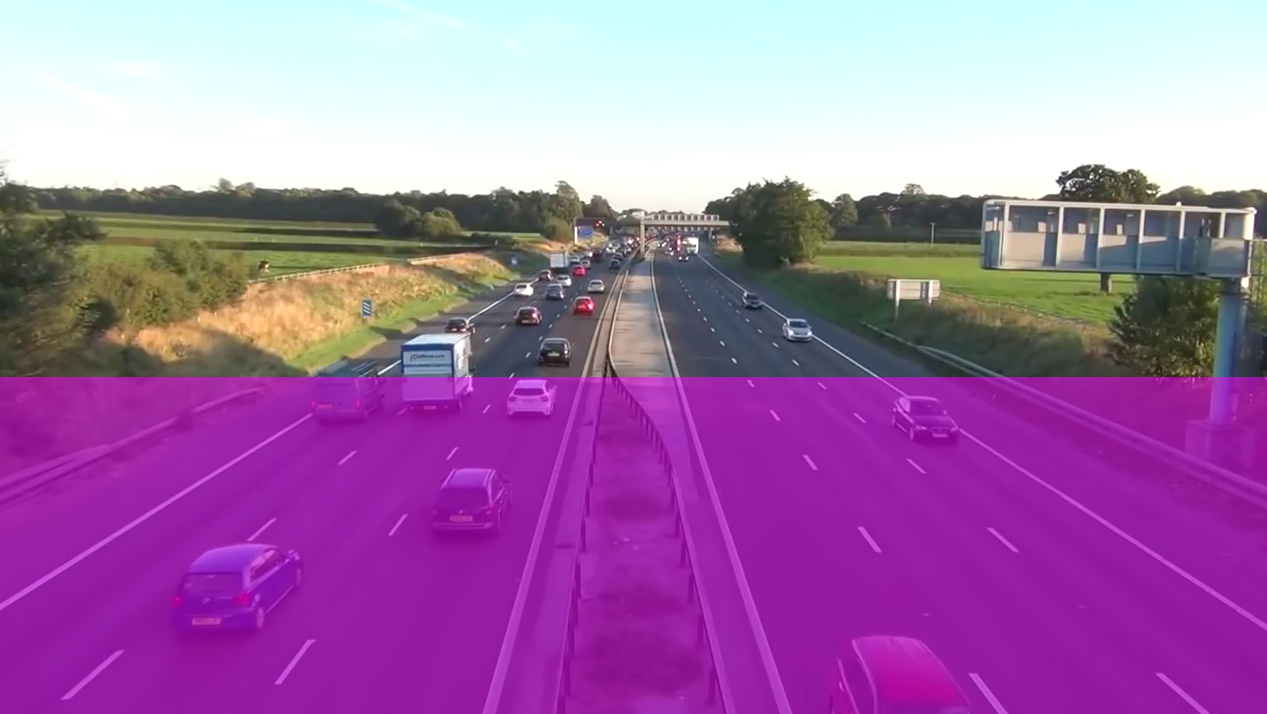
\includegraphics[width = 0.8\textwidth]{design/detection/counting/original_speed}
	\caption{Visualization of speed measurement region.}
	\label{fig:speed}
\end{figure} 

\subsubsection{Calibration}

The calibration of these two components is critical to the utility of the overall system because if the data that is being collected is not accurate then the system is redundant. Central to this calibration process is the selection of a region of interest which is predicated on an area of the image that is returning the best vehicle recognition, the counting line and speed measuring region should be placed within this region of interest. Were this line to be placed in a region where many false vehicle recognitions occurred then it would incur many false positive counts and likewise were it placed where vehicles are not recognised it would incur false negatives. This line is calibrated by visually analysing where centroids are being most consistently and correctly tracked and verified by comparing manual counts of traffic in test videos against the counts obtained by the system. 

The speed estimation calibration requires a conversion from pixels to meters that can be determined by knowing some dimension of an object in the frame in the real world. Furthermore, to improve the consistency of speed measurements only vehicles that have a centroid history featuring position recording in four sectors of the overall speed region can contribute to the statistics. Figure \ref{fig:speed_sectors} fives a visualization of these sectors.

\begin{figure}[H]
	\centering
	\centering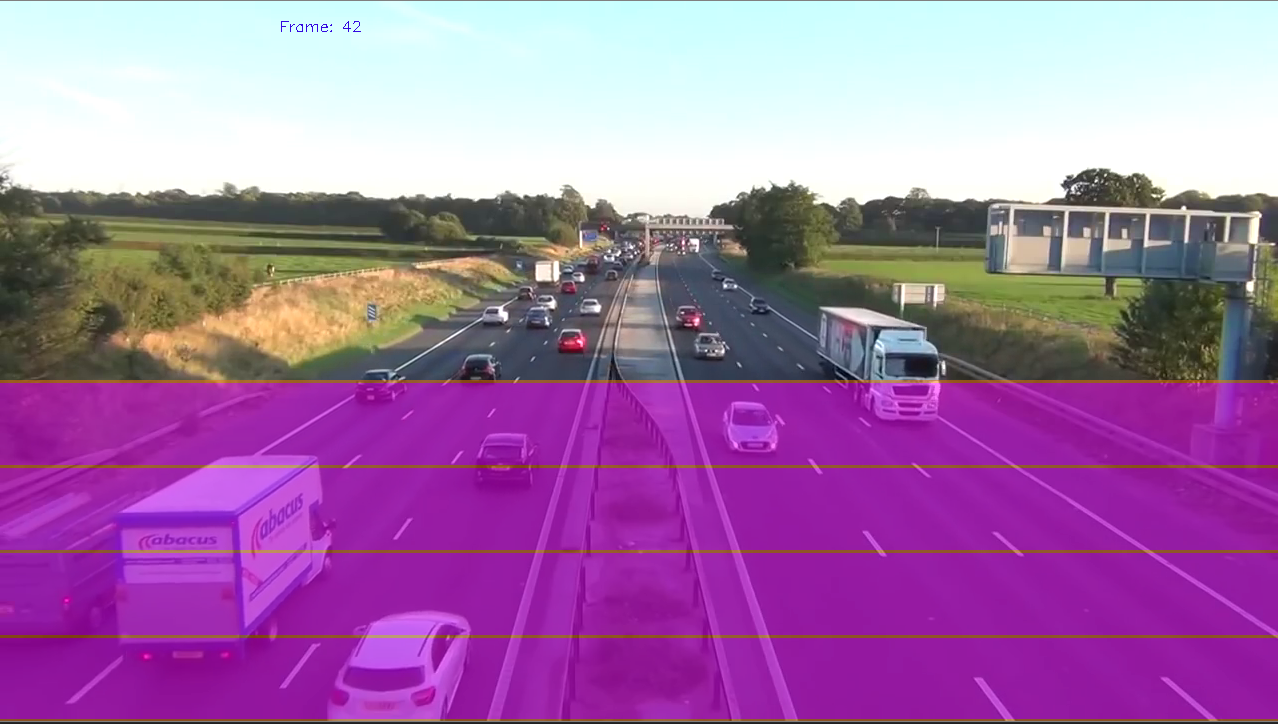
\includegraphics[width = 0.8\textwidth]{design/detection/counting/speed_sectors}
	\caption{Visualization of four speed sectors of a speed region.}
	\label{fig:speed_sectors}
  \end{figure}
  